\documentclass{beamer}

\usepackage{subfig}
\usepackage{hyperref}
\usepackage{csquotes}
\usepackage[Q=yes]{examplep}

\hypersetup{
    colorlinks=true,
    linkcolor=blue,
    filecolor=magenta,      
    urlcolor=cyan,
}

\mode<presentation> {
    \usetheme{Madrid}
}

\title[\textcolor{white}{Vim - Fun and Efficient}]{\huge Vim \\
    \large Making text editing fun and efficient
}

\author{Alec Gibson}
\institute[BlueCat]
{
    BlueCat Networks \\
    \medskip
    \textit{agibson@bluecatnetworks.com}
}
\date{November 24, 2020}

\begin{document}

\begin{frame}[fragile]
    \titlepage % Print the title page as the first slide
\end{frame}

\begin{frame}[fragile]
    \frametitle{Disclaimer}
    \small The target audience of this talk is not seasoned users of Vi-family editors (though you are more than welcome to stay if this describes you). Many of the features I will refer to as Vim features were Vi features first. I never used Vi, and clarifying when features were introduced in Vim's lineage is outside the scope of this talk. So for the purpose of this talk they are Vim features.\\
    \vspace{0.5cm}
    Furthermore, almost everything I say in this talk applies equally to Neovim as it does to Vim. Neovim is a fork of Vim with slightly tweaked default options, no Benevolent Dictator For Life, and which tends to implement new features more quickly. I personally use Neovim instead of Vim, but both operate extremely similarly.
\end{frame}

\begin{frame}[fragile]
    \frametitle{About This Presentation}
    \begin{itemize}
	\item This presentation was created in Neovim 0.5.0 using the Beamer Latex package
	\item The source code is available at \url{https://github.com/alec-gibson/vim-fun-and-efficient}
	\item For discussions about Vim, please post in the company \#vim-geeks slack channel!
    \end{itemize}
\end{frame}

\begin{frame}[fragile]
    \frametitle{Overview}
    \tableofcontents
\end{frame}

\section{About Vim}

\begin{frame}[fragile]
    \frametitle{About Vim}
    \tableofcontents[currentsection]
\end{frame}

\begin{frame}[fragile]
    \frametitle{What is Vim}
    \centerline{\large According to vim.org}
    \vspace{0.5cm}
    \small Vim is a highly configurable text editor built to make creating and changing any kind of text very efficient. It is included as \enquote{vi} with most UNIX systems and with Apple OS X.\\
    \vspace{0.5cm}
    Vim is rock stable and is continuously being developed to become even better. Among its features are:\\
    \begin{itemize}
	\item persistent, multi-level undo tree
	\item extensive plugin system
	\item support for hundreds of programming languages and file formats
	\item powerful search and replace
	\item integrates with many tools
    \end{itemize}
\end{frame}

\begin{frame}[fragile]
    \centerline{\large Here are some important features I think were missed:}
    \vspace{0.5cm}
    \small
    \begin{itemize}
	\item Vim is very lightweight, meaning it runs smoothly on any modern computer and performs well over SSH.
	\item Vim's startup time is nearly instantaneous.
	\item Because Vim runs in a terminal it works nicely with other terminal utilities (like tmux), and you can pipe the output of scripts directly into Vim.
	\item Vim's configuration is scriptable, so you can define custom functions then use them in commands and keybindings.
	\item Once you learn Vim you can use it everywhere - its keybindings are supported in most other editors either natively or through plugins (including VSCode, Emacs, and IntelliJ to name a few)
    \end{itemize}
\end{frame}

\begin{frame}[fragile]
    \centerline{\large And most importantly....}
    \vspace{0.5cm}
    \small \textbf{If you are not already using them, Vim's keybindings can teach you a new, more efficient way to edit text.}\\
\end{frame}

\begin{frame}[fragile]
    \frametitle{Who Should Try Vim?}
    \centerline{\large You may appreciate Vim if you:}
    \vspace{0.5cm}
    \begin{itemize}
	\item Spend a large amount of your day editing plain text files (common in software development and IT)
	\item Make frequent use of your terminal emulator
	\item Appreciate the value of keyboard shortcuts for everything
	\item Like to customize your tools to suit your workflow
	\item \textbf{And especially} if you spend too much time making boring, repetitive edits
    \end{itemize}
\end{frame}

\section{A Minimal Vim Workflow}

\begin{frame}[fragile]
    \frametitle{A Minimal Vim Workflow}
    \tableofcontents[currentsection]
\end{frame}

\begin{frame}[fragile]
    \frametitle{Modal Editing}
    \small
    \begin{block}{Modal Editing}
	Vim is a modal text editor, meaning keypresses in Vim perform different actions depending upon the editor's current \enquote{mode}.\\
    \end{block}
    When you edit a file in Vim, the editor starts in \enquote{normal} mode. This can confuse new users, because Vim's normal mode treats every key on the keyboard as a binding for a shortcut. To start off learning Vim, let's look at the smallest possible set of features you need to edit files.
\end{frame}

\begin{frame}[fragile]
    \frametitle{Basic Vim File Operations}
    \small
    \begin{itemize}
	\item To open a file in Vim, type \verb+vim {filename}+ in your terminal emulator.
	\item To change the current open file, type \verb+:e /path/to/file<CR>+.
	\item To save the current file, type \verb+:w<CR>+.
	\item Finally, to exit Vim type \verb+:q<CR>+.
    \end{itemize}
    \begin{block}{What's That CR Symbol?}
	\verb+<CR>+ is how you represent the Enter/Return key in Vim keybindings.
    \end{block}
    \begin{block}{Popular Variants}
	Popular variants of these commands include \verb+:wq<CR>+ to save and quit, and \verb+:wq!<CR>+ to force Vim to save and quit (ignoring any warnings while doing so).
    \end{block}
\end{frame}

\begin{frame}[fragile]
    \frametitle{Basic Vim Editing}
    \small
    The simplest (though probably the slowest) way to navigate a file in Vim is using the arrow keys. To make changes in the current file, press \verb+i+ to enter \enquote{insert} mode. In insert mode, keys behave the way they would in any other text editor - letter and number keys insert their corresponding characters, and \verb+<BS>+ (backspace) deletes the previous character. \\
    \vspace{0.5cm}
    If you want to run any of the file operations from the previous slide, just press \verb+<ESC>+ (escape) to return to normal mode first.
    \begin{block}{Using Your Mouse in Vim!?}
	It's true, Vim supports using your mouse. Just set the required option by typing \verb+:set mouse=a+ in normal mode.
    \end{block}
\end{frame}

\begin{frame}[fragile]
    \small This is about as much of Vim as some people ever learn. It's enough to edit config files on servers over SSH (albeit slowly), or to use while setting up a minimal Linux installation on a PC. \\
    \vspace{0.5cm}
    However, if this was the most efficient way to edit files in Vim, \textbf{the editor would have died out long ago}.
\end{frame}

\section{Vim Can Do More}

\begin{frame}[fragile]
    \frametitle{Vim Can Do More}
    \tableofcontents[currentsection]
\end{frame}

\begin{frame}[fragile]
    \frametitle{Why The Minimal Workflow Isn't Enough}
    \small
    The minimal Vim workflow I described in the previous section is seriously inefficient. Here are a few reasons why:
    \begin{itemize}
	\item Using the mouse requires you to take your right hand off the keyboard
	\item Using the arrow keys requires you to take your right hand off the home row
	\item You can only move one character at a time using the arrow keys
	\item You can only delete one character at a time using \verb+<BS>+
	\item If your cursor is in the middle of some text, you have to move to the end to delete it
	\item We don't have any way to copy and paste
	\item We don't have a way to undo mistakes
	\item This workflow doesn't include any way to search the current file
	\item Repeated edits need to be executed manually each time
    \end{itemize}
    Vim's normal mode has features which solve all these issues.
\end{frame}

\begin{frame}[fragile]
    \frametitle{Movement Keybindings}
    \small
    \begin{block}{Problem}
	\begin{itemize}
	    \item Using the mouse requires you to take your right hand off the keyboard
	    \item Using the arrow keys requires you to take your right hand off the home row
	\end{itemize}
    \end{block}
    Vim solves these issues by using the keys \verb+h, j, k, and l+ as alternatives to the arrow keys while in normal mode. These behave in the following manner:
    \begin{description}
	\item[h] Move left one character
	\item[j] Move down one character
	\item[k] Move up one character
	\item[l] Move right one character
    \end{description}
    These keybindings are well-known enough that other programs which also use hjkl for navigation often refer to them as \enquote{Vim keys}.
\end{frame}

\begin{frame}[fragile]
    \frametitle{Moving Longer Distances}
    \small
    \begin{block}{Problem}
	\begin{itemize}
	    \item You can only move one character at a time using the arrow keys
	\end{itemize}
    \end{block}
    Vim's normal mode contains many keybindings for moving more than one character at a time. Here are some I use frequently:
    \begin{itemize}
	\item \verb+w/b+:  Move forward/back by one word at a time
	\item \verb+0/$+:  Move to the start/end of the current line (use \verb+^+ instead of 0 to move to the first non-whitespace character of the line)
	\item \verb+<C-d>+/\verb+<C-u>+:  Move down/up by half a screen at a time
	\item \verb+gg/G+:  Move to the start/end of the current file
    \end{itemize}
    \begin{block}{Useful Keybindings: f and F}
	Typing f\{char\} searches the current line for the chosen character, and using F searches backwards. Pressing \enquote{;} jumps to the next occurrence, and pressing \enquote{,} goes to the previous occurence (very useful if you overshoot your target). This is often the fastest way to jump to a specific location on the current line.
    \end{block}
\end{frame}

\begin{frame}[fragile]
    \begin{block}{Repeating Movements Multiple Times}
	Most Vim commands allow you to prepend a number to multiply their effects. For example:
	\begin{itemize}
	    \item typing \verb+5j+ in normal mode moves your cursor down 5 lines.
	    \item typing \verb+3w+ moves your cursor forward 3 words
	    \item typing \verb+10fe+ moves your cursor to the tenth occurence of the character \enquote{e} following it on the current line
	\end{itemize}
    \end{block}
\end{frame}

\begin{frame}[fragile]
    \frametitle{Keybindings for Editing}
    Vim has a number of keybindings for editing the current file's contents. We can start with keybindings which operate on single characters:
    \begin{itemize}
	\item \verb+x+:  delete the character under the cursor
	\item \verb+r{char}+:  replace the character under the cursor with \{char\}
	\item \verb+~+:  swap the case of the character under the cursor
	\item \verb+<C-a>+/\verb+<C-x>+:  increment / decrement the number under the cursor
    \end{itemize}
\end{frame}

\begin{frame}[fragile]
    \frametitle{Operating on Chunks of Text}
    \begin{block}{Problem}
	\begin{itemize}
	    \item You can only delete one character at a time using \verb+<BS>+
	\end{itemize}
    \end{block}
    Operating on chunks of text is where Vim's keybinding system really shines. Vim separates these edits into keybindings it calls \enquote{operators} and \enquote{motions}.
    \begin{block}{Operators}
	Operators are the verbs of the edit - they are things like \enquote{delete}, \enquote{change}, \enquote{yank} (Vim language for \enquote{copy}), \enquote{indent}, \enquote{format}, etc.
    \end{block}
    \begin{block}{Motions}
	Motions are like nouns - they define what the operator should operate on. Examples of motions would be \enquote{a word}, \enquote{until the end of the line}, or \enquote{to the end of the file}.
    \end{block}
\end{frame}

\begin{frame}[fragile]
    Operators:
    \begin{itemize}
	\item \verb+d+:  delete
	\item \verb+c+:  change (delete, then enter insert mode)
	\item \verb+y+:  yank (copy)
	\item \verb+<+/\verb+>+:  increase / decrease indent
	\item \verb+=+:  format (works well for C-style languages, but is configurable)
    \end{itemize}
\end{frame}

\begin{frame}[fragile]
    Example Edits:
    \begin{itemize}
	\item \verb+dl+:  delete to the right (same as x)
	\item \verb+dh+:  delete to the left
	\item \verb+dw+:  delete word
	\item \verb+c$+:  change to the end of the line
	\item \verb+yG+:  yank to the end of the file
	\item \verb+dt_+:  delete to the next underscore $\ast$
    \end{itemize}
    Note: \verb+t+ and \verb+T+ act like \verb+f+ and \verb+F+, but they stop one character before the character being search for. These are extremely useful for operating on all the text before a certain target character. \verb+snake_case+, \verb+kebab-case+ and \verb+camelCase+ are used frequently in source code files, so it often works well to make your target character the next underscore, hypen, or a specific capital letter.
\end{frame}

\begin{frame}[fragile]
    \begin{block}{Shortcuts for Common Operations}
	There are also some special editing keybindings to make frequently required editing operations more convenient. Repeating the operator twice means to apply it to the current line (\verb+dd+ deletes the current line, \verb+yy+ yanks the current line, etc.). There are also shortcuts for when you capitalize the operators - \verb+D+ deletes to the end of the line, \verb+Y+ is equivalent to \verb+yy+, etc.
    \end{block}
\end{frame}

\begin{frame}[fragile]
    For most motions, the easiest way to understand the behaviour of Vim edits is to imagine the behaviour of the cursor if you typed the motion without the operator, then the operator will be applied to the characters spanned by that motion. This is why, for example, \verb+dw+ doesn't delete the entire word the cursor is currently inside, but rather deletes from the current cursor position to the beginning of the next word.\\
    \vspace{0.5cm}
    Sometimes this is not the behaviour we want - sometimes we want to delete the entire word the cursor is currently inside. We will explore how to do this using \enquote{text objects} on the next slide.
\end{frame}

\begin{frame}[fragile]
    \frametitle{Text Objects}
    \begin{block}{Problem}
	\begin{itemize}
	    \item If your cursor is in the middle of some text, you have to move to the end to delete it
	\end{itemize}
    \end{block}
    Up until now, the motions we have applied to operators have also been normal mode navigation keybindings. This is not always the case. After typing the operator but before the motion, Vim is in a special mode called \enquote{operator-pending} mode, and this mode has some of its own unique keybindings. Text objects are an example of keybindings for operator-pending mode. These keybindings let operators work on an area of text the cursor is already inside - for example the current word or the surrounding set of quotation marks.
\end{frame}

\begin{frame}[fragile]
    examples of text objects:
    \begin{itemize}
	\item \verb+iw/aw+: inner / around word
	\item \verb+is/as+: inner / around sentence
	\item \verb+ip/ap+: inner / around paragraph
	\item \verb+i"/a"+: inner / around quoted string
	\item \verb+i(/a(+: inner / around \verb+()+ block
	\item \verb+i[/a[+: inner / around \verb+[]+ block
	\item \verb+i{/a{+: inner / around \verb+{}+ block
    \end{itemize}
    Language plugins often add text objects, for example to operate on the contents of classes and functions.
\end{frame}

\begin{frame}[fragile]
    Each of the \enquote{inner} variants of the provided text objects ignore whitespace and surrounding delimiters. The \enquote{around} variants include the surrounding delimiters and whitespace. \\
    \vspace{0.5cm}
    For example, \verb+di"+ will delete the contents of the quotation marks the cursor is currently inside, but will not touch the quotation marks themselves. In contrast, \verb+da"+ will delete the contents of the quotation marks, the quotation marks, and surrounding whitespace. \\
    \vspace{0.5cm}
    To frame this differently, if you had a series of quoted strings separated by spaces, \verb+di"+ would delete the contents of the current string, but repeating it again would do nothing. In contrast, \verb+da"+ would delete the current quoted string, so that the cursor is now on the next quoted string, so if you repeated the edit it would deleted each quoted string in turn.
\end{frame}

\begin{frame}[fragile]
    \frametitle{Pasting, or \enquote{Putting}}
    \begin{block}{Problem}
	\begin{itemize}
	    \item We don't have any way to copy and paste
	\end{itemize}
    \end{block}
    We've seen how to yank text already using the \verb+y+ operator. Now all you need to do to \enquote{put} it (Vim language for pasting) is to press \verb+p+.\\
    \vspace{0.5cm}
    It is important to know, deleting in Vim does not just delete the chosen text, but behaves more like the \enquote{cut} operation in other popular editors. That is to say, the deleted text will be the next thing \enquote{put} when the user presses \verb+p+. We will look at ways to get around this later in the Vim Power Tools section, when we discuss registers.
\end{frame}

\begin{frame}[fragile]
    \frametitle{Searching}
    \begin{block}{Problem}
	\begin{itemize}
	    \item This workflow doesn't include any way to search the current file
	\end{itemize}
    \end{block}
    Searching is very quick in Vim, and is often the fastest way to navigate a file. Press \verb+/+ to initiate a search, then type in the pattern to search for (patterns are regular expressions so, among other things, they can include wildcards) and press \verb+<CR>+ to start the search. To move to the next search result press \verb+n+ and to move to the previous result press \verb+N+. Here are a few other useful keybindings for searching:
    \begin{itemize}
	\item \verb+?+: start a search in the opposite direction
	\item \verb+q/+: view a history of previous search patterns (press \verb+<CR>+ on one to search for it in the current file)
	\item \verb+/<CR>+: search again using the most recently used search pattern
    \end{itemize}
\end{frame}

\begin{frame}[fragile]
    \frametitle{Undo and Redo}
    \begin{block}{Problem}
	\begin{itemize}
	    \item We don't have a way to undo mistakes
	\end{itemize}
    \end{block}
    You can undo the most recent edit by pressing \verb+u+, and you can press \verb+u+ multiple times to continue undoing edits. An example of a single \enquote{edit} in Vim would be a single operator + motion combination. Everything you type from pressing \verb+i+ to enter insert mode until returning to normal mode is considered a single edit, so pressing \verb+u+ once will undo all of it.\\
    \vspace{0.5cm}
    You can press \verb+<C-r>+ to "redo" the most recently undone edit. Like with \verb+u+, you can repeatedly press \verb+<C-r>+ to redo more undone edits.\\
    \vspace{0.5cm}
    If you accidentally undo too much then edit the document, it is still possible to recover - Vim keeps track of your branching undos. We'll discuss this later in the Vim Power Tools section when we discuss the Undo Tree.
\end{frame}

\begin{frame}[fragile]
    \frametitle{Repeating Edits}
    \begin{block}{Problem}
	\begin{itemize}
	    \item Repeated edits need to be executed manually each time
	\end{itemize}
    \end{block}
    We discussed on the previous slide what a single \enquote{edit} is in Vim. You can repeat the most recent edit by pressing the \verb+.+ key.\\
    \vspace{0.5cm}
    Effectively using \verb+.+ takes a lot of practice, and requires that you plan your edits to be repeatable. For example, if you run \verb+diw+ to delete a word, then \verb+i+ to enter insert mode and type its replacement, subsequent presses of \verb+.+ will perform the insertion but not the deletion. If you want the deletion to be included in the repeated edit, you could use \verb+ciw+ instead.\\
    \vspace{0.5cm}
    Vim supports many ways to repeat edits. I'll discuss macros, \verb+:substitute+ and \verb+:global+ in the \enquote{Power Tools} section of this talk. All of these are more flexible than the \verb+.+ key.
\end{frame}

\begin{frame}[fragile]
    \frametitle{How to Find Help}
    Vim comes with extensive documentation built-in, accessible using the \verb+:h+ command (short for \verb+:help+, which works too if you want to be verbose). If you want to look up what a particular keybinding does, you can run \verb+:h {key}<CR>+ to look up the corresponding help file. If you don't know the name of the help file you are looking for, you can run \verb+:helpgrep {phrase}<CR>+ to search all Vim's help files for a particular phrase. Helpgrep fills Vim's \enquote{quickfix} list with its results - we will discuss the quickfix list more later, but for now just know you can run \verb+:cnext<CR>+ to go to the next result and \verb+:cprev<CR>+ to go to the previous result.
\end{frame}

\begin{frame}[fragile]
    \frametitle{How to Learn Vim}
    If you want more thorough materials to learn Vim, you can start by running \verb+vimtutor+ in your terminal (it usually comes with your installation of Vim). After completing vimtutor, you can read Vim's user manual for a lengthy but readable guide to all of Vim's most important features. To read the user manual, run \verb+:h user-manual<CR>+ in Vim.
\end{frame}

\section{Power Tools}

\begin{frame}[fragile]
    \frametitle{Power Tools}
    \tableofcontents[currentsection]
\end{frame}

\begin{frame}[fragile]
    Now that we've covered most of the basic features of Vim, you have seen one of the reasons many developers swear by it as their editor of choice - the ability to modularly compose edits using operators and navigation keybindings gives you a very terse language for quickly editing documents. However, there are probably still some people wondering \textbf{why would anyone want to use this editor}? Hopefully the features I discuss in this section will help make a stronger case in favour of Vim.
\end{frame}

\begin{frame}[fragile]
    To start with, I'll cover Command-Line Mode and Visual Mode to round out our understanding of Vim's modes. Then we'll get into some of (what I consider) Vim's killer features - the jump list, registers, macros, \verb+:substitute+, \verb+:global+, and the undo tree. By the end of this section I'll have explained enough of Vim's features that, if you became fluent in their usage, you could edit single files in Vim quite efficiently. \\
    \vspace{0.5cm}
    After this section, we'll cover ways to manage editing multiple files in a single Vim session, then we'll finish up with a short introduction to Vim configuration.
\end{frame}

\begin{frame}[fragile]
    \frametitle{Command-Line Mode}
    Many of Vim's features are accessible using keybindings in normal mode. However, we can also access features by writing out the names of commands to execute using Vim's command-line mode. Press \verb+:+ to enter command-line mode, then you can type in the name of a command and hit \verb+<CR>+ to execute it and return to normal mode. If you change your mind, you can press \verb+<ESC>+ to go back to normal mode without executing a command.\\
    \vspace{0.5cm}
    \begin{block}{We've Seen This Before}
	We have already learned several Vim command-line mode commands. The file operations we learned (\verb+:w+, \verb+:q+ and \verb+:e+) all execute in command-line mode, as do the \verb+:h+ and \verb+:helpgrep+ commands. Vim doesn't require you to type the whole name of a command to execute it - you just need to type enough to disambiguate it from other commands. The file operations we learned are actually short forms for \verb+:write+, \verb+:quit+ and \verb+:edit+.
    \end{block}
\end{frame}

\begin{frame}[fragile]
    \begin{block}{How do I See My Command-Line History?}
	When you are in command-line mode, you can press the up and down arrow keys (or \verb+<C-p>+ and \verb+<C-n>+, emacs style) to select previously run commands. You can view your command-line history by typing \verb+q:+ in normal mode. This will open a window showing past commands you've run, where you can edit a previous command, then execute the edited version using \verb+<CR>+.
    \end{block}
\end{frame}

\begin{frame}[fragile]
    \frametitle{Visual Mode}
    One of the disadvantages of Vim's operator + motion syntax for defining an edit, is that you need to decide on the appropriate motion for an edit on the spot after already commiting to an operator. If you would prefer to make your selection of text to operate on first, then specify the operator after, Vim contains three different \enquote{visual modes} which allow you to do just that.
    \begin{block}{Character-Wise Visual Mode}
	The simplest visual mode Vim offers is character-wise visual mode, often just refered to as visual mode. You can enter this visual mode by pressing \verb+v+, and exit to normal mode using \verb+<ESC>+. While in any visual mode, your current text selection will be highlighted. You can move the cursor to change where the visual selection ends, or press \verb+o+ to instead change where the selection starts. After making your selection you can use operators on the selected text, like \verb+d+ to delete it, or \verb+y+ to yank it.
    \end{block}
\end{frame}

\begin{frame}[fragile]
    \begin{block}{Line-Wise Visual Mode}
	You can press \verb+V+ (capital V) to enter line-wise visual mode - a variant of visual mode which only selects entire lines. I often use this version of visual mode to delete or yank data which is formatted into separate lines, such as a function, a JSON object, or a chunk of YAML. It is also useful for constraining the scope of some command-line commands, something we'll explore more when we discuss the \verb+:substitute+ command.
    \end{block}
    \begin{block}{Block-Wise Visual Mode}
	You can press \verb+<C-v>+ to enter block-wise visual mode, which lets you select a rectangular region of text. I have found this most useful when I want to add, remove or modify a prefix for several lines. For example, if I wanted to create a bulleted list, I would use block-wise visual mode to select the first character of several lines, press \verb+I+ to insert at the start of each line's selection in the block (a special block-wise visual mode mapping), type \verb+-+, then press \verb+<ESC>+. Upon returning to normal mode, all my selected lines would be updated to begin with a hyphen.
    \end{block}
\end{frame}

\begin{frame}[fragile]
    \frametitle{The Jump List}
    This is a simple feature, but it is \textbf{constantly} useful, and I wish every text editor had it. Vim keeps track of every time you use a motion to move a significant distance, and stores these locations you've jumped to in its \enquote{jump list}. You can view this jump list by running the \verb+:jumps+ command.\\
    \vspace{0.5cm}
    The useful part is that Vim lets you jump back to older locations you've been using \verb+<C-o>+ and newer locations using \verb+<C-i>+. This means for example, if you created a tags file using ctags, you could jump to a function's definition using \verb+<C-]>+. Then, using the jump list you could use \verb+<C-o>+ to jump back to where the function is called when you're done looking at it. I use this functionality constantly when reading new code I haven't seen before.\\
    \vspace{0.5cm}
    Note: the \verb+<C-]>+ keybinding also lets you jump to referenced help pages inside \verb+:help+.
\end{frame}

\begin{frame}[fragile]
    \frametitle{Registers}
\end{frame}

\begin{frame}[fragile]
    \frametitle{Macros}
\end{frame}

\begin{frame}[fragile]
    \frametitle{:substitute}
\end{frame}

\begin{frame}[fragile]
    \frametitle{:global}
\end{frame}

\begin{frame}[fragile]
    \frametitle{:normal}
\end{frame}

\begin{frame}[fragile]
    \frametitle{The Undo Tree}
\end{frame}

\section{Managing and Editing Multiple Files}

\begin{frame}[fragile]
    \frametitle{Managing and Editing Multiple Files}
    \tableofcontents[currentsection]
\end{frame}

\begin{frame}[fragile]
    \frametitle{Buffers, Windows and Tabs}
\end{frame}

\begin{frame}[fragile]
    \frametitle{Argument, Location and Quickfix Lists}
\end{frame}

\begin{frame}[fragile]
    \frametitle{Grep and Vimgrep}
\end{frame}

\begin{frame}[fragile]
    \frametitle{Cdo, Ldo, Argdo}
\end{frame}

\begin{frame}[fragile]
    \frametitle{Finding Files Quickly}
    NOTE: discuss fuzzy finder and file tree plugins here
\end{frame}

\section{Configuration}

\begin{frame}[fragile]
    \frametitle{Configuration}
    \tableofcontents[currentsection]
\end{frame}

\begin{frame}[fragile]
    \frametitle{Setting Options}
\end{frame}

\begin{frame}[fragile]
    \frametitle{Keybindings}
\end{frame}

\begin{frame}[fragile]
    \frametitle{Abbreviations}
\end{frame}

\begin{frame}[fragile]
    \frametitle{Functions}
\end{frame}

\begin{frame}[fragile]
    \frametitle{Custom Commands}
\end{frame}

\begin{frame}[fragile]
    \frametitle{Automatic Commands}
\end{frame}

\begin{frame}[fragile]
    \frametitle{Plugins}
\end{frame}

\section{Links for Further Learning}

\begin{frame}[fragile]
    \frametitle{Links for Further Learning}
\end{frame}

\section{Goodbye}

\begin{frame}[fragile]
    \centerline{\huge All Praise VI VI VI}
    \vspace{0.5cm}
    \centerline{\huge Editor of The Beast}
    \begin{figure}
	\centering
	\subfloat{{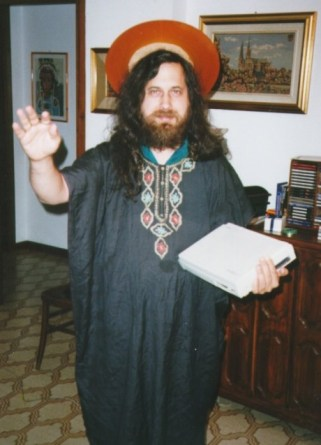
\includegraphics[width=0.3\linewidth]{saintignucius.jpg} }}% Created by Wouter van Oortmerssen
	\qquad
	\subfloat{{
\includegraphics[width=0.3\linewidth]{freebsd-daemon.png} }}% Created by Poul-Henning Kamp under the beer-ware license (https://svnweb.freebsd.org/base/head/share/examples/BSD_daemon/README?view=markup)
    \end{figure}
\end{frame}

\end{document} 
